% Created by tikzDevice version 0.12.6 on 2026-09-11 15:07:18
% !TEX encoding = UTF-8 Unicode
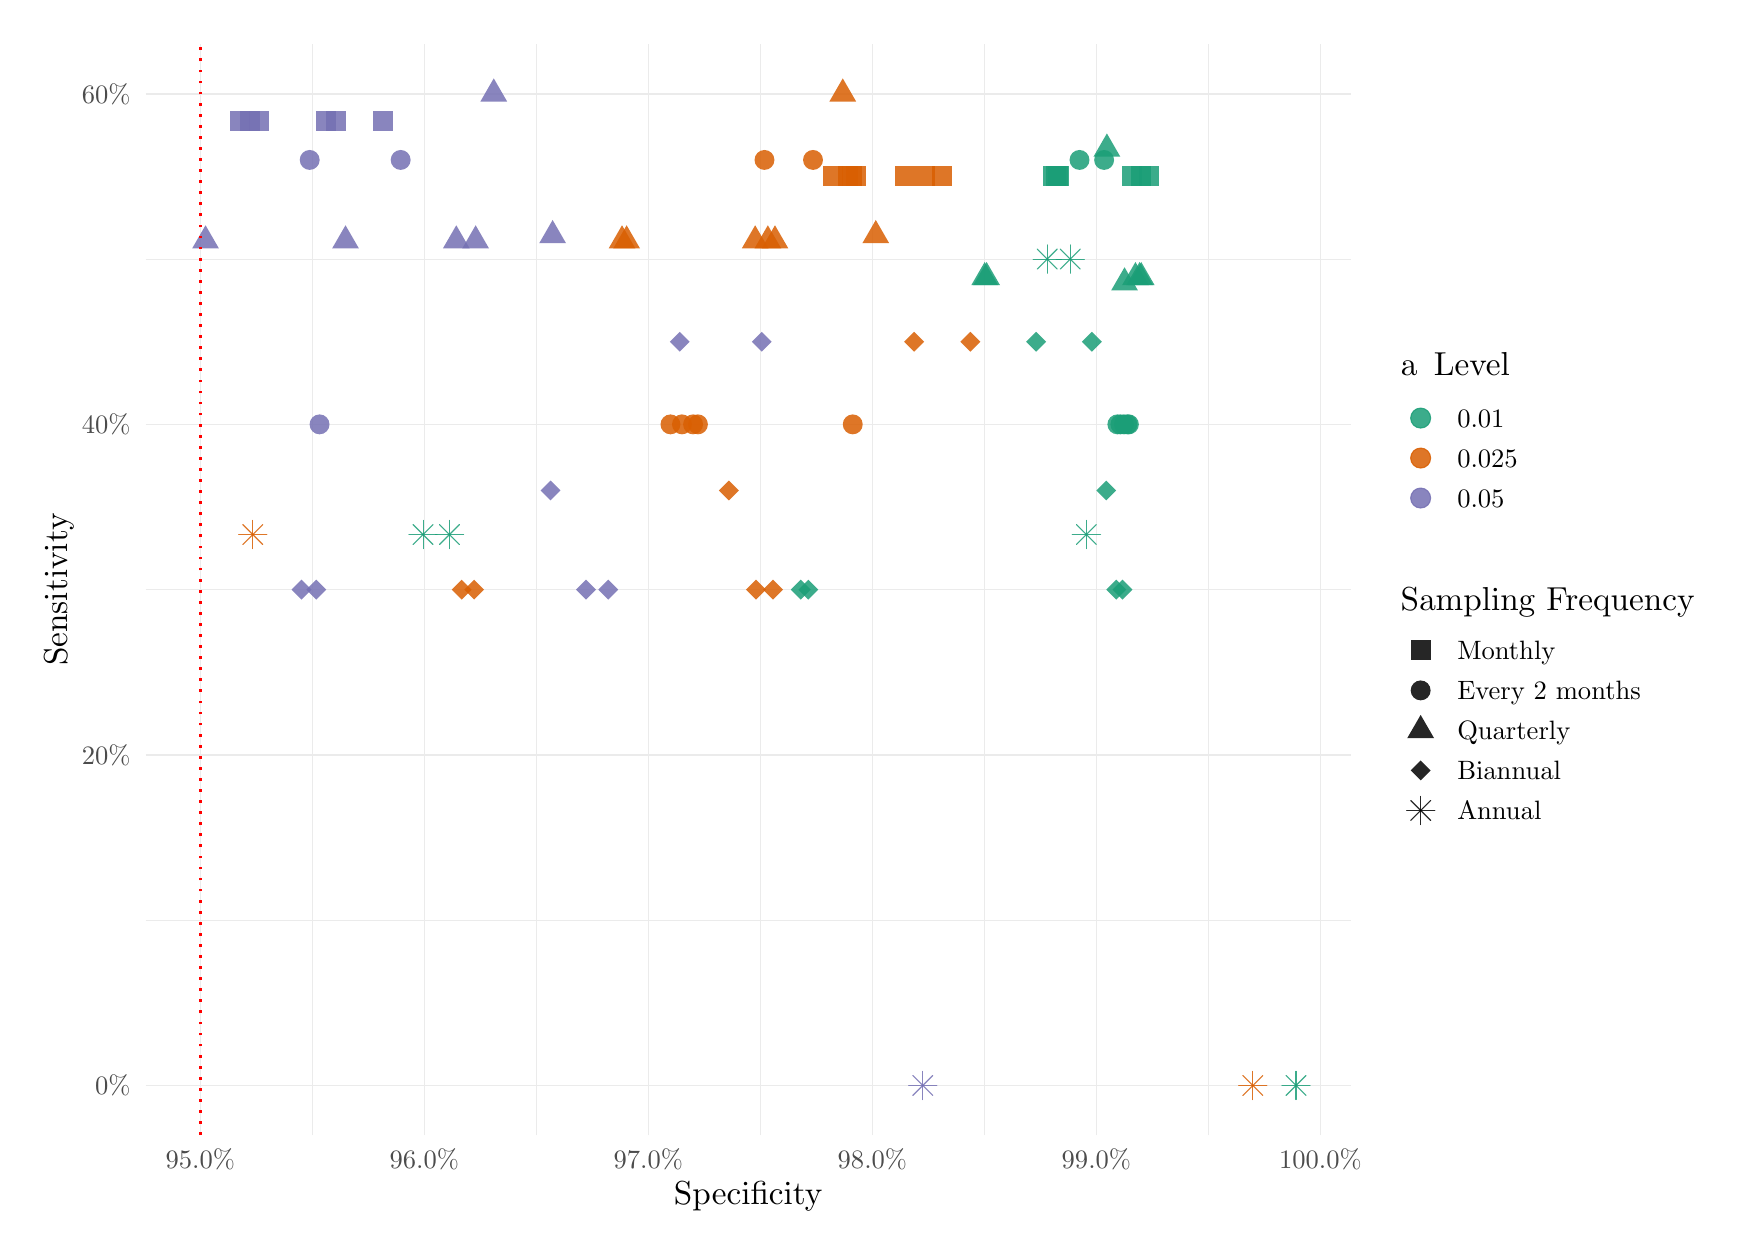
\begin{tikzpicture}[x=1pt,y=1pt]
\definecolor{fillColor}{RGB}{255,255,255}
\path[use as bounding box,fill=fillColor,fill opacity=0.00] (0,0) rectangle (614.29,433.62);
\begin{scope}
\path[clip] (  0.00,  0.00) rectangle (614.29,433.62);
\definecolor{fillColor}{RGB}{255,255,255}

\path[fill=fillColor] ( -0.00,  0.00) rectangle (614.29,433.62);
\end{scope}
\begin{scope}
\path[clip] ( 42.59, 33.48) rectangle (478.12,427.62);
\definecolor{drawColor}{gray}{0.92}

\path[draw=drawColor,line width= 0.3pt,line join=round] ( 42.59,111.11) --
	(478.12,111.11);

\path[draw=drawColor,line width= 0.3pt,line join=round] ( 42.59,230.55) --
	(478.12,230.55);

\path[draw=drawColor,line width= 0.3pt,line join=round] ( 42.59,349.99) --
	(478.12,349.99);

\path[draw=drawColor,line width= 0.3pt,line join=round] (102.86, 33.48) --
	(102.86,427.62);

\path[draw=drawColor,line width= 0.3pt,line join=round] (183.81, 33.48) --
	(183.81,427.62);

\path[draw=drawColor,line width= 0.3pt,line join=round] (264.76, 33.48) --
	(264.76,427.62);

\path[draw=drawColor,line width= 0.3pt,line join=round] (345.71, 33.48) --
	(345.71,427.62);

\path[draw=drawColor,line width= 0.3pt,line join=round] (426.65, 33.48) --
	(426.65,427.62);

\path[draw=drawColor,line width= 0.6pt,line join=round] ( 42.59, 51.39) --
	(478.12, 51.39);

\path[draw=drawColor,line width= 0.6pt,line join=round] ( 42.59,170.83) --
	(478.12,170.83);

\path[draw=drawColor,line width= 0.6pt,line join=round] ( 42.59,290.27) --
	(478.12,290.27);

\path[draw=drawColor,line width= 0.6pt,line join=round] ( 42.59,409.70) --
	(478.12,409.70);

\path[draw=drawColor,line width= 0.6pt,line join=round] ( 62.39, 33.48) --
	( 62.39,427.62);

\path[draw=drawColor,line width= 0.6pt,line join=round] (143.34, 33.48) --
	(143.34,427.62);

\path[draw=drawColor,line width= 0.6pt,line join=round] (224.28, 33.48) --
	(224.28,427.62);

\path[draw=drawColor,line width= 0.6pt,line join=round] (305.23, 33.48) --
	(305.23,427.62);

\path[draw=drawColor,line width= 0.6pt,line join=round] (386.18, 33.48) --
	(386.18,427.62);

\path[draw=drawColor,line width= 0.6pt,line join=round] (467.13, 33.48) --
	(467.13,427.62);
\definecolor{fillColor}{RGB}{117,112,179}

\path[fill=fillColor,fill opacity=0.85] ( 79.97,396.15) --
	( 87.17,396.15) --
	( 87.17,403.35) --
	( 79.97,403.35) --
	cycle;

\path[fill=fillColor,fill opacity=0.85] ( 76.67,396.15) --
	( 83.87,396.15) --
	( 83.87,403.35) --
	( 76.67,403.35) --
	cycle;

\path[fill=fillColor,fill opacity=0.85] ( 73.22,396.15) --
	( 80.42,396.15) --
	( 80.42,403.35) --
	( 73.22,403.35) --
	cycle;

\path[fill=fillColor,fill opacity=0.85] (104.22,396.15) --
	(111.42,396.15) --
	(111.42,403.35) --
	(104.22,403.35) --
	cycle;

\path[fill=fillColor,fill opacity=0.85] (124.66,396.15) --
	(131.86,396.15) --
	(131.86,403.35) --
	(124.66,403.35) --
	cycle;

\path[fill=fillColor,fill opacity=0.85] (107.80,396.15) --
	(115.00,396.15) --
	(115.00,403.35) --
	(107.80,403.35) --
	cycle;

\path[fill=fillColor,fill opacity=0.85] (105.47,290.27) circle (  3.60);

\path[fill=fillColor,fill opacity=0.85] (134.78,385.82) circle (  3.60);

\path[fill=fillColor,fill opacity=0.85] (101.91,385.82) circle (  3.60);

\path[fill=fillColor,fill opacity=0.85] ( 64.27,362.22) --
	( 69.12,353.82) --
	( 59.42,353.82) --
	cycle;

\path[fill=fillColor,fill opacity=0.85] (114.85,362.22) --
	(119.70,353.82) --
	(110.00,353.82) --
	cycle;

\path[fill=fillColor,fill opacity=0.85] (161.87,362.22) --
	(166.72,353.82) --
	(157.02,353.82) --
	cycle;

\path[fill=fillColor,fill opacity=0.85] (154.88,362.22) --
	(159.73,353.82) --
	(150.03,353.82) --
	cycle;

\path[fill=fillColor,fill opacity=0.85] (189.69,364.12) --
	(194.54,355.72) --
	(184.84,355.72) --
	cycle;

\path[fill=fillColor,fill opacity=0.85] (168.42,415.30) --
	(173.27,406.90) --
	(163.57,406.90) --
	cycle;

\path[fill=fillColor,fill opacity=0.85] (100.70,230.55) --
	(104.30,234.15) --
	(107.90,230.55) --
	(104.30,226.95) --
	cycle;

\path[fill=fillColor,fill opacity=0.85] ( 95.36,230.55) --
	( 98.96,234.15) --
	(102.56,230.55) --
	( 98.96,226.95) --
	cycle;

\path[fill=fillColor,fill opacity=0.85] (206.19,230.55) --
	(209.79,234.15) --
	(213.39,230.55) --
	(209.79,226.95) --
	cycle;

\path[fill=fillColor,fill opacity=0.85] (198.15,230.55) --
	(201.75,234.15) --
	(205.35,230.55) --
	(201.75,226.95) --
	cycle;

\path[fill=fillColor,fill opacity=0.85] (185.33,266.38) --
	(188.93,269.98) --
	(192.53,266.38) --
	(188.93,262.78) --
	cycle;

\path[fill=fillColor,fill opacity=0.85] (261.65,320.13) --
	(265.25,323.73) --
	(268.85,320.13) --
	(265.25,316.53) --
	cycle;

\path[fill=fillColor,fill opacity=0.85] (232.02,320.13) --
	(235.62,323.73) --
	(239.22,320.13) --
	(235.62,316.53) --
	cycle;
\definecolor{drawColor}{RGB}{117,112,179}

\path[draw=drawColor,draw opacity=0.85,line width= 0.4pt,line join=round,line cap=round] (319.84, 47.79) -- (327.05, 54.99);

\path[draw=drawColor,draw opacity=0.85,line width= 0.4pt,line join=round,line cap=round] (319.84, 54.99) -- (327.05, 47.79);

\path[draw=drawColor,draw opacity=0.85,line width= 0.4pt,line join=round,line cap=round] (318.35, 51.39) -- (328.54, 51.39);

\path[draw=drawColor,draw opacity=0.85,line width= 0.4pt,line join=round,line cap=round] (323.45, 46.30) -- (323.45, 56.48);
\definecolor{fillColor}{RGB}{217,95,2}

\path[fill=fillColor,fill opacity=0.85] (287.49,376.24) --
	(294.69,376.24) --
	(294.69,383.45) --
	(287.49,383.45) --
	cycle;

\path[fill=fillColor,fill opacity=0.85] (295.57,376.24) --
	(302.77,376.24) --
	(302.77,383.45) --
	(295.57,383.45) --
	cycle;

\path[fill=fillColor,fill opacity=0.85] (294.18,376.24) --
	(301.38,376.24) --
	(301.38,383.45) --
	(294.18,383.45) --
	cycle;

\path[fill=fillColor,fill opacity=0.85] (292.67,376.24) --
	(299.87,376.24) --
	(299.87,383.45) --
	(292.67,383.45) --
	cycle;

\path[fill=fillColor,fill opacity=0.85] (326.65,376.24) --
	(333.86,376.24) --
	(333.86,383.45) --
	(326.65,383.45) --
	cycle;

\path[fill=fillColor,fill opacity=0.85] (320.60,376.24) --
	(327.80,376.24) --
	(327.80,383.45) --
	(320.60,383.45) --
	cycle;

\path[fill=fillColor,fill opacity=0.85] (313.49,376.24) --
	(320.69,376.24) --
	(320.69,383.45) --
	(313.49,383.45) --
	cycle;

\path[fill=fillColor,fill opacity=0.85] (242.20,290.27) circle (  3.60);

\path[fill=fillColor,fill opacity=0.85] (240.44,290.27) circle (  3.60);

\path[fill=fillColor,fill opacity=0.85] (236.42,290.27) circle (  3.60);

\path[fill=fillColor,fill opacity=0.85] (232.27,290.27) circle (  3.60);

\path[fill=fillColor,fill opacity=0.85] (298.14,290.27) circle (  3.60);

\path[fill=fillColor,fill opacity=0.85] (283.78,385.82) circle (  3.60);

\path[fill=fillColor,fill opacity=0.85] (266.24,385.82) circle (  3.60);

\path[fill=fillColor,fill opacity=0.85] (216.43,362.22) --
	(221.28,353.82) --
	(211.58,353.82) --
	cycle;

\path[fill=fillColor,fill opacity=0.85] (214.77,362.22) --
	(219.62,353.82) --
	(209.92,353.82) --
	cycle;

\path[fill=fillColor,fill opacity=0.85] (270.03,362.22) --
	(274.88,353.82) --
	(265.18,353.82) --
	cycle;

\path[fill=fillColor,fill opacity=0.85] (267.46,362.22) --
	(272.31,353.82) --
	(262.61,353.82) --
	cycle;

\path[fill=fillColor,fill opacity=0.85] (262.88,362.22) --
	(267.73,353.82) --
	(258.03,353.82) --
	cycle;

\path[fill=fillColor,fill opacity=0.85] (306.46,364.12) --
	(311.31,355.72) --
	(301.61,355.72) --
	cycle;

\path[fill=fillColor,fill opacity=0.85] (294.53,415.30) --
	(299.38,406.90) --
	(289.68,406.90) --
	cycle;

\path[fill=fillColor,fill opacity=0.85] (157.72,230.55) --
	(161.32,234.15) --
	(164.92,230.55) --
	(161.32,226.95) --
	cycle;

\path[fill=fillColor,fill opacity=0.85] (153.22,230.55) --
	(156.82,234.15) --
	(160.42,230.55) --
	(156.82,226.95) --
	cycle;

\path[fill=fillColor,fill opacity=0.85] (265.74,230.55) --
	(269.34,234.15) --
	(272.94,230.55) --
	(269.34,226.95) --
	cycle;

\path[fill=fillColor,fill opacity=0.85] (259.56,230.55) --
	(263.16,234.15) --
	(266.76,230.55) --
	(263.16,226.95) --
	cycle;

\path[fill=fillColor,fill opacity=0.85] (249.76,266.38) --
	(253.36,269.98) --
	(256.96,266.38) --
	(253.36,262.78) --
	cycle;

\path[fill=fillColor,fill opacity=0.85] (337.02,320.13) --
	(340.62,323.73) --
	(344.22,320.13) --
	(340.62,316.53) --
	cycle;

\path[fill=fillColor,fill opacity=0.85] (316.69,320.13) --
	(320.29,323.73) --
	(323.89,320.13) --
	(320.29,316.53) --
	cycle;
\definecolor{drawColor}{RGB}{217,95,2}

\path[draw=drawColor,draw opacity=0.85,line width= 0.4pt,line join=round,line cap=round] ( 77.75,246.85) -- ( 84.95,254.05);

\path[draw=drawColor,draw opacity=0.85,line width= 0.4pt,line join=round,line cap=round] ( 77.75,254.05) -- ( 84.95,246.85);

\path[draw=drawColor,draw opacity=0.85,line width= 0.4pt,line join=round,line cap=round] ( 76.26,250.45) -- ( 86.44,250.45);

\path[draw=drawColor,draw opacity=0.85,line width= 0.4pt,line join=round,line cap=round] ( 81.35,245.36) -- ( 81.35,255.55);

\path[draw=drawColor,draw opacity=0.85,line width= 0.4pt,line join=round,line cap=round] (439.11, 47.79) -- (446.31, 54.99);

\path[draw=drawColor,draw opacity=0.85,line width= 0.4pt,line join=round,line cap=round] (439.11, 54.99) -- (446.31, 47.79);

\path[draw=drawColor,draw opacity=0.85,line width= 0.4pt,line join=round,line cap=round] (437.61, 51.39) -- (447.80, 51.39);

\path[draw=drawColor,draw opacity=0.85,line width= 0.4pt,line join=round,line cap=round] (442.71, 46.30) -- (442.71, 56.48);
\definecolor{fillColor}{RGB}{27,158,119}

\path[fill=fillColor,fill opacity=0.85] (368.91,376.24) --
	(376.11,376.24) --
	(376.11,383.45) --
	(368.91,383.45) --
	cycle;

\path[fill=fillColor,fill opacity=0.85] (368.60,376.24) --
	(375.80,376.24) --
	(375.80,383.45) --
	(368.60,383.45) --
	cycle;

\path[fill=fillColor,fill opacity=0.85] (367.82,376.24) --
	(375.02,376.24) --
	(375.02,383.45) --
	(367.82,383.45) --
	cycle;

\path[fill=fillColor,fill opacity=0.85] (366.96,376.24) --
	(374.17,376.24) --
	(374.17,383.45) --
	(366.96,383.45) --
	cycle;

\path[fill=fillColor,fill opacity=0.85] (401.57,376.24) --
	(408.77,376.24) --
	(408.77,383.45) --
	(401.57,383.45) --
	cycle;

\path[fill=fillColor,fill opacity=0.85] (398.63,376.24) --
	(405.83,376.24) --
	(405.83,383.45) --
	(398.63,383.45) --
	cycle;

\path[fill=fillColor,fill opacity=0.85] (395.40,376.24) --
	(402.60,376.24) --
	(402.60,383.45) --
	(395.40,383.45) --
	cycle;

\path[fill=fillColor,fill opacity=0.85] (397.92,290.27) circle (  3.60);

\path[fill=fillColor,fill opacity=0.85] (397.36,290.27) circle (  3.60);

\path[fill=fillColor,fill opacity=0.85] (396.12,290.27) circle (  3.60);

\path[fill=fillColor,fill opacity=0.85] (394.84,290.27) circle (  3.60);

\path[fill=fillColor,fill opacity=0.85] (393.76,290.27) circle (  3.60);

\path[fill=fillColor,fill opacity=0.85] (388.97,385.82) circle (  3.60);

\path[fill=fillColor,fill opacity=0.85] (380.08,385.82) circle (  3.60);

\path[fill=fillColor,fill opacity=0.85] (346.52,348.95) --
	(351.37,340.55) --
	(341.67,340.55) --
	cycle;

\path[fill=fillColor,fill opacity=0.85] (345.81,348.95) --
	(350.66,340.55) --
	(340.96,340.55) --
	cycle;

\path[fill=fillColor,fill opacity=0.85] (402.38,348.95) --
	(407.23,340.55) --
	(397.53,340.55) --
	cycle;

\path[fill=fillColor,fill opacity=0.85] (401.79,348.95) --
	(406.64,340.55) --
	(396.94,340.55) --
	cycle;

\path[fill=fillColor,fill opacity=0.85] (400.29,348.95) --
	(405.14,340.55) --
	(395.44,340.55) --
	cycle;

\path[fill=fillColor,fill opacity=0.85] (396.35,347.05) --
	(401.20,338.65) --
	(391.50,338.65) --
	cycle;

\path[fill=fillColor,fill opacity=0.85] (389.97,395.40) --
	(394.82,387.00) --
	(385.13,387.00) --
	cycle;

\path[fill=fillColor,fill opacity=0.85] (278.49,230.55) --
	(282.09,234.15) --
	(285.69,230.55) --
	(282.09,226.95) --
	cycle;

\path[fill=fillColor,fill opacity=0.85] (275.77,230.55) --
	(279.37,234.15) --
	(282.97,230.55) --
	(279.37,226.95) --
	cycle;

\path[fill=fillColor,fill opacity=0.85] (392.00,230.55) --
	(395.60,234.15) --
	(399.20,230.55) --
	(395.60,226.95) --
	cycle;

\path[fill=fillColor,fill opacity=0.85] (389.76,230.55) --
	(393.36,234.15) --
	(396.96,230.55) --
	(393.36,226.95) --
	cycle;

\path[fill=fillColor,fill opacity=0.85] (386.14,266.38) --
	(389.74,269.98) --
	(393.34,266.38) --
	(389.74,262.78) --
	cycle;

\path[fill=fillColor,fill opacity=0.85] (380.94,320.13) --
	(384.54,323.73) --
	(388.14,320.13) --
	(384.54,316.53) --
	cycle;

\path[fill=fillColor,fill opacity=0.85] (360.79,320.13) --
	(364.39,323.73) --
	(367.99,320.13) --
	(364.39,316.53) --
	cycle;
\definecolor{drawColor}{RGB}{27,158,119}

\path[draw=drawColor,draw opacity=0.85,line width= 0.4pt,line join=round,line cap=round] (148.81,246.85) -- (156.01,254.05);

\path[draw=drawColor,draw opacity=0.85,line width= 0.4pt,line join=round,line cap=round] (148.81,254.05) -- (156.01,246.85);

\path[draw=drawColor,draw opacity=0.85,line width= 0.4pt,line join=round,line cap=round] (147.32,250.45) -- (157.51,250.45);

\path[draw=drawColor,draw opacity=0.85,line width= 0.4pt,line join=round,line cap=round] (152.41,245.36) -- (152.41,255.55);

\path[draw=drawColor,draw opacity=0.85,line width= 0.4pt,line join=round,line cap=round] (139.27,246.85) -- (146.48,254.05);

\path[draw=drawColor,draw opacity=0.85,line width= 0.4pt,line join=round,line cap=round] (139.27,254.05) -- (146.48,246.85);

\path[draw=drawColor,draw opacity=0.85,line width= 0.4pt,line join=round,line cap=round] (137.78,250.45) -- (147.97,250.45);

\path[draw=drawColor,draw opacity=0.85,line width= 0.4pt,line join=round,line cap=round] (142.87,245.36) -- (142.87,255.55);

\path[draw=drawColor,draw opacity=0.85,line width= 0.4pt,line join=round,line cap=round] (378.95,246.85) -- (386.16,254.05);

\path[draw=drawColor,draw opacity=0.85,line width= 0.4pt,line join=round,line cap=round] (378.95,254.05) -- (386.16,246.85);

\path[draw=drawColor,draw opacity=0.85,line width= 0.4pt,line join=round,line cap=round] (377.46,250.45) -- (387.65,250.45);

\path[draw=drawColor,draw opacity=0.85,line width= 0.4pt,line join=round,line cap=round] (382.55,245.36) -- (382.55,255.55);

\path[draw=drawColor,draw opacity=0.85,line width= 0.4pt,line join=round,line cap=round] (373.13,346.38) -- (380.33,353.59);

\path[draw=drawColor,draw opacity=0.85,line width= 0.4pt,line join=round,line cap=round] (373.13,353.59) -- (380.33,346.38);

\path[draw=drawColor,draw opacity=0.85,line width= 0.4pt,line join=round,line cap=round] (371.64,349.99) -- (381.82,349.99);

\path[draw=drawColor,draw opacity=0.85,line width= 0.4pt,line join=round,line cap=round] (376.73,344.89) -- (376.73,355.08);

\path[draw=drawColor,draw opacity=0.85,line width= 0.4pt,line join=round,line cap=round] (364.79,346.38) -- (371.99,353.59);

\path[draw=drawColor,draw opacity=0.85,line width= 0.4pt,line join=round,line cap=round] (364.79,353.59) -- (371.99,346.38);

\path[draw=drawColor,draw opacity=0.85,line width= 0.4pt,line join=round,line cap=round] (363.30,349.99) -- (373.49,349.99);

\path[draw=drawColor,draw opacity=0.85,line width= 0.4pt,line join=round,line cap=round] (368.39,344.89) -- (368.39,355.08);

\path[draw=drawColor,draw opacity=0.85,line width= 0.4pt,line join=round,line cap=round] (454.72, 47.79) -- (461.93, 54.99);

\path[draw=drawColor,draw opacity=0.85,line width= 0.4pt,line join=round,line cap=round] (454.72, 54.99) -- (461.93, 47.79);

\path[draw=drawColor,draw opacity=0.85,line width= 0.4pt,line join=round,line cap=round] (453.23, 51.39) -- (463.42, 51.39);

\path[draw=drawColor,draw opacity=0.85,line width= 0.4pt,line join=round,line cap=round] (458.32, 46.30) -- (458.32, 56.48);
\definecolor{drawColor}{RGB}{255,0,0}

\path[draw=drawColor,line width= 1.1pt,dash pattern=on 1pt off 3pt ,line join=round] ( 62.39, 33.48) -- ( 62.39,427.62);
\end{scope}
\begin{scope}
\path[clip] (  0.00,  0.00) rectangle (614.29,433.62);
\definecolor{drawColor}{gray}{0.30}

\node[text=drawColor,anchor=base east,inner sep=0pt, outer sep=0pt, scale=  0.96] at ( 37.19, 48.09) {0\%};

\node[text=drawColor,anchor=base east,inner sep=0pt, outer sep=0pt, scale=  0.96] at ( 37.19,167.52) {20\%};

\node[text=drawColor,anchor=base east,inner sep=0pt, outer sep=0pt, scale=  0.96] at ( 37.19,286.96) {40\%};

\node[text=drawColor,anchor=base east,inner sep=0pt, outer sep=0pt, scale=  0.96] at ( 37.19,406.40) {60\%};
\end{scope}
\begin{scope}
\path[clip] (  0.00,  0.00) rectangle (614.29,433.62);
\definecolor{drawColor}{gray}{0.30}

\node[text=drawColor,anchor=base,inner sep=0pt, outer sep=0pt, scale=  0.96] at ( 62.39, 21.46) {95.0\%};

\node[text=drawColor,anchor=base,inner sep=0pt, outer sep=0pt, scale=  0.96] at (143.34, 21.46) {96.0\%};

\node[text=drawColor,anchor=base,inner sep=0pt, outer sep=0pt, scale=  0.96] at (224.28, 21.46) {97.0\%};

\node[text=drawColor,anchor=base,inner sep=0pt, outer sep=0pt, scale=  0.96] at (305.23, 21.46) {98.0\%};

\node[text=drawColor,anchor=base,inner sep=0pt, outer sep=0pt, scale=  0.96] at (386.18, 21.46) {99.0\%};

\node[text=drawColor,anchor=base,inner sep=0pt, outer sep=0pt, scale=  0.96] at (467.13, 21.46) {100.0\%};
\end{scope}
\begin{scope}
\path[clip] (  0.00,  0.00) rectangle (614.29,433.62);
\definecolor{drawColor}{RGB}{0,0,0}

\node[text=drawColor,anchor=base,inner sep=0pt, outer sep=0pt, scale=  1.20] at (260.36,  8.33) {Specificity};
\end{scope}
\begin{scope}
\path[clip] (  0.00,  0.00) rectangle (614.29,433.62);
\definecolor{drawColor}{RGB}{0,0,0}

\node[text=drawColor,rotate= 90.00,anchor=base,inner sep=0pt, outer sep=0pt, scale=  1.20] at ( 14.26,230.55) {Sensitivity};
\end{scope}
\begin{scope}
\path[clip] (  0.00,  0.00) rectangle (614.29,433.62);
\definecolor{drawColor}{RGB}{0,0,0}

\node[text=drawColor,anchor=base west,inner sep=0pt, outer sep=0pt, scale=  1.20] at (496.12,308.11) {a};

\node[text=drawColor,anchor=base west,inner sep=0pt, outer sep=0pt, scale=  1.20] at (502.12,308.11) { };

\node[text=drawColor,anchor=base west,inner sep=0pt, outer sep=0pt, scale=  1.20] at (508.12,308.11) {Level};
\end{scope}
\begin{scope}
\path[clip] (  0.00,  0.00) rectangle (614.29,433.62);
\definecolor{drawColor}{RGB}{27,158,119}
\definecolor{fillColor}{RGB}{27,158,119}

\path[draw=drawColor,draw opacity=0.85,line width= 0.4pt,line join=round,line cap=round,fill=fillColor,fill opacity=0.85] (503.35,292.55) circle (  3.60);
\end{scope}
\begin{scope}
\path[clip] (  0.00,  0.00) rectangle (614.29,433.62);
\definecolor{drawColor}{RGB}{217,95,2}
\definecolor{fillColor}{RGB}{217,95,2}

\path[draw=drawColor,draw opacity=0.85,line width= 0.4pt,line join=round,line cap=round,fill=fillColor,fill opacity=0.85] (503.35,278.10) circle (  3.60);
\end{scope}
\begin{scope}
\path[clip] (  0.00,  0.00) rectangle (614.29,433.62);
\definecolor{drawColor}{RGB}{117,112,179}
\definecolor{fillColor}{RGB}{117,112,179}

\path[draw=drawColor,draw opacity=0.85,line width= 0.4pt,line join=round,line cap=round,fill=fillColor,fill opacity=0.85] (503.35,263.65) circle (  3.60);
\end{scope}
\begin{scope}
\path[clip] (  0.00,  0.00) rectangle (614.29,433.62);
\definecolor{drawColor}{RGB}{0,0,0}

\node[text=drawColor,anchor=base west,inner sep=0pt, outer sep=0pt, scale=  0.96] at (516.58,289.25) {0.01};
\end{scope}
\begin{scope}
\path[clip] (  0.00,  0.00) rectangle (614.29,433.62);
\definecolor{drawColor}{RGB}{0,0,0}

\node[text=drawColor,anchor=base west,inner sep=0pt, outer sep=0pt, scale=  0.96] at (516.58,274.79) {0.025};
\end{scope}
\begin{scope}
\path[clip] (  0.00,  0.00) rectangle (614.29,433.62);
\definecolor{drawColor}{RGB}{0,0,0}

\node[text=drawColor,anchor=base west,inner sep=0pt, outer sep=0pt, scale=  0.96] at (516.58,260.34) {0.05};
\end{scope}
\begin{scope}
\path[clip] (  0.00,  0.00) rectangle (614.29,433.62);
\definecolor{drawColor}{RGB}{0,0,0}

\node[text=drawColor,anchor=base west,inner sep=0pt, outer sep=0pt, scale=  1.20] at (496.12,222.99) {Sampling Frequency};
\end{scope}
\begin{scope}
\path[clip] (  0.00,  0.00) rectangle (614.29,433.62);
\definecolor{fillColor}{RGB}{0,0,0}

\path[fill=fillColor,fill opacity=0.85] (499.75,204.99) --
	(506.95,204.99) --
	(506.95,212.20) --
	(499.75,212.20) --
	cycle;
\end{scope}
\begin{scope}
\path[clip] (  0.00,  0.00) rectangle (614.29,433.62);
\definecolor{fillColor}{RGB}{0,0,0}

\path[fill=fillColor,fill opacity=0.85] (503.35,194.14) circle (  3.60);
\end{scope}
\begin{scope}
\path[clip] (  0.00,  0.00) rectangle (614.29,433.62);
\definecolor{fillColor}{RGB}{0,0,0}

\path[fill=fillColor,fill opacity=0.85] (503.35,185.29) --
	(508.20,176.89) --
	(498.50,176.89) --
	cycle;
\end{scope}
\begin{scope}
\path[clip] (  0.00,  0.00) rectangle (614.29,433.62);
\definecolor{fillColor}{RGB}{0,0,0}

\path[fill=fillColor,fill opacity=0.85] (499.75,165.23) --
	(503.35,168.83) --
	(506.95,165.23) --
	(503.35,161.63) --
	cycle;
\end{scope}
\begin{scope}
\path[clip] (  0.00,  0.00) rectangle (614.29,433.62);
\definecolor{drawColor}{RGB}{0,0,0}

\path[draw=drawColor,draw opacity=0.85,line width= 0.4pt,line join=round,line cap=round] (499.75,147.18) -- (506.95,154.38);

\path[draw=drawColor,draw opacity=0.85,line width= 0.4pt,line join=round,line cap=round] (499.75,154.38) -- (506.95,147.18);

\path[draw=drawColor,draw opacity=0.85,line width= 0.4pt,line join=round,line cap=round] (498.26,150.78) -- (508.44,150.78);

\path[draw=drawColor,draw opacity=0.85,line width= 0.4pt,line join=round,line cap=round] (503.35,145.69) -- (503.35,155.87);
\end{scope}
\begin{scope}
\path[clip] (  0.00,  0.00) rectangle (614.29,433.62);
\definecolor{drawColor}{RGB}{0,0,0}

\node[text=drawColor,anchor=base west,inner sep=0pt, outer sep=0pt, scale=  0.96] at (516.58,205.29) {Monthly};
\end{scope}
\begin{scope}
\path[clip] (  0.00,  0.00) rectangle (614.29,433.62);
\definecolor{drawColor}{RGB}{0,0,0}

\node[text=drawColor,anchor=base west,inner sep=0pt, outer sep=0pt, scale=  0.96] at (516.58,190.83) {Every 2 months};
\end{scope}
\begin{scope}
\path[clip] (  0.00,  0.00) rectangle (614.29,433.62);
\definecolor{drawColor}{RGB}{0,0,0}

\node[text=drawColor,anchor=base west,inner sep=0pt, outer sep=0pt, scale=  0.96] at (516.58,176.38) {Quarterly};
\end{scope}
\begin{scope}
\path[clip] (  0.00,  0.00) rectangle (614.29,433.62);
\definecolor{drawColor}{RGB}{0,0,0}

\node[text=drawColor,anchor=base west,inner sep=0pt, outer sep=0pt, scale=  0.96] at (516.58,161.93) {Biannual};
\end{scope}
\begin{scope}
\path[clip] (  0.00,  0.00) rectangle (614.29,433.62);
\definecolor{drawColor}{RGB}{0,0,0}

\node[text=drawColor,anchor=base west,inner sep=0pt, outer sep=0pt, scale=  0.96] at (516.58,147.47) {Annual};
\end{scope}
\end{tikzpicture}
